



\documentclass[12pt]{article}

\usepackage[brazil]{babel}
\usepackage[utf8]{inputenc}
\usepackage{graphicx}
\usepackage{float}
\usepackage{indentfirst}

\title{Estudo sobre artistas importantes para conexão entre a banda Raça Negra e grupos similares}
\author{
	Marcelo Gianfaldoni de Andrade\\
	Engenharia da Computação\\
	Insper\\
}
\date{\today}


\begin{document}
\maketitle

\newpage
\tableofcontents
\newpage

\begin{abstract}
Esse artigo busca fazer um estudo sobre bandas centrais para a conexão entre diferentes grupos de artistas relacionados à banda Raça Negra. Para esse estudo, será feita uma análise a partir das recomendações entre bandas cadastradas no serviço Spotify usando como ponto inicial o Raça Negra. A partir dos dados coletados, irá ser feito um grafo e uma análise de centralidade nos nós do mesmo para, enfim, encontrar os melhores candidatos para bandas centrais nesse cenário tão complexo culturalmente. Ao fim, será mostrado as dez bandas consideradas mais centrais a partir das considerações iniciais.
\end{abstract}

\section{Introdução}
Embora a música popular brasileira seja conhecido como um gênero musical isolado, pode-se considerar outros inúmeros estilos musicais como parte dessa categoria: samba, sertanejo, pagode, funk, bossa nova, axé, etc.

Com tantos estilos musicais presentes em um gênero, é difícil reconhecer os artistas que estão nas fronteiras entre essas categorias, nesse caso específico, relacionados ao Raça Negra. Portanto, esse estudo busca responder a seguinte questão: Quais são os artistas mais importantes na conexão entre diferentes grupos formados por bandas relacionadas ao Raça Negra? Sejam esses grupos gêneros musicais ou outras possíveis classificações.

Ao final do estudo, foi possível listar dez bandas que respondem essa pergunta. Esse resultado possibilita um melhor entendimento das fronteiras nebulosas entre bandas de estilos diferentes. Uma possível aplicação desse conhecimento seria uma recomendação desses artistas para ouvintes de grupos próximos a estes que buscam novos gostos musicais. 

\section{Método utilizado}
Para obtenção dos dados necessários, foi-se escolhido usar a API do Spotify, por conter grande partes dos artistas mais famosos do país e apresentar uma característica que permite a criação de um grafo; a recomendação de um artista para outro.

A partir dessas características do serviço, teve-se que escolher um artista como ponto de partida para se criar uma rede de conexões a partir do mesmo. Foi escolhido arbitrariamente o grupo Raça Negra, por ser um importantíssimo grupo musical na cultura popular brasileira e ao mesmo tempo apresentar muitas recomendações no Spotify. Com os dados coletados, criou-se um grafo com os artistas como nós e uma aresta entre dois nós sempre que a recomendação entre eles fosse mútua.

\begin{figure}[H]
	\centering
	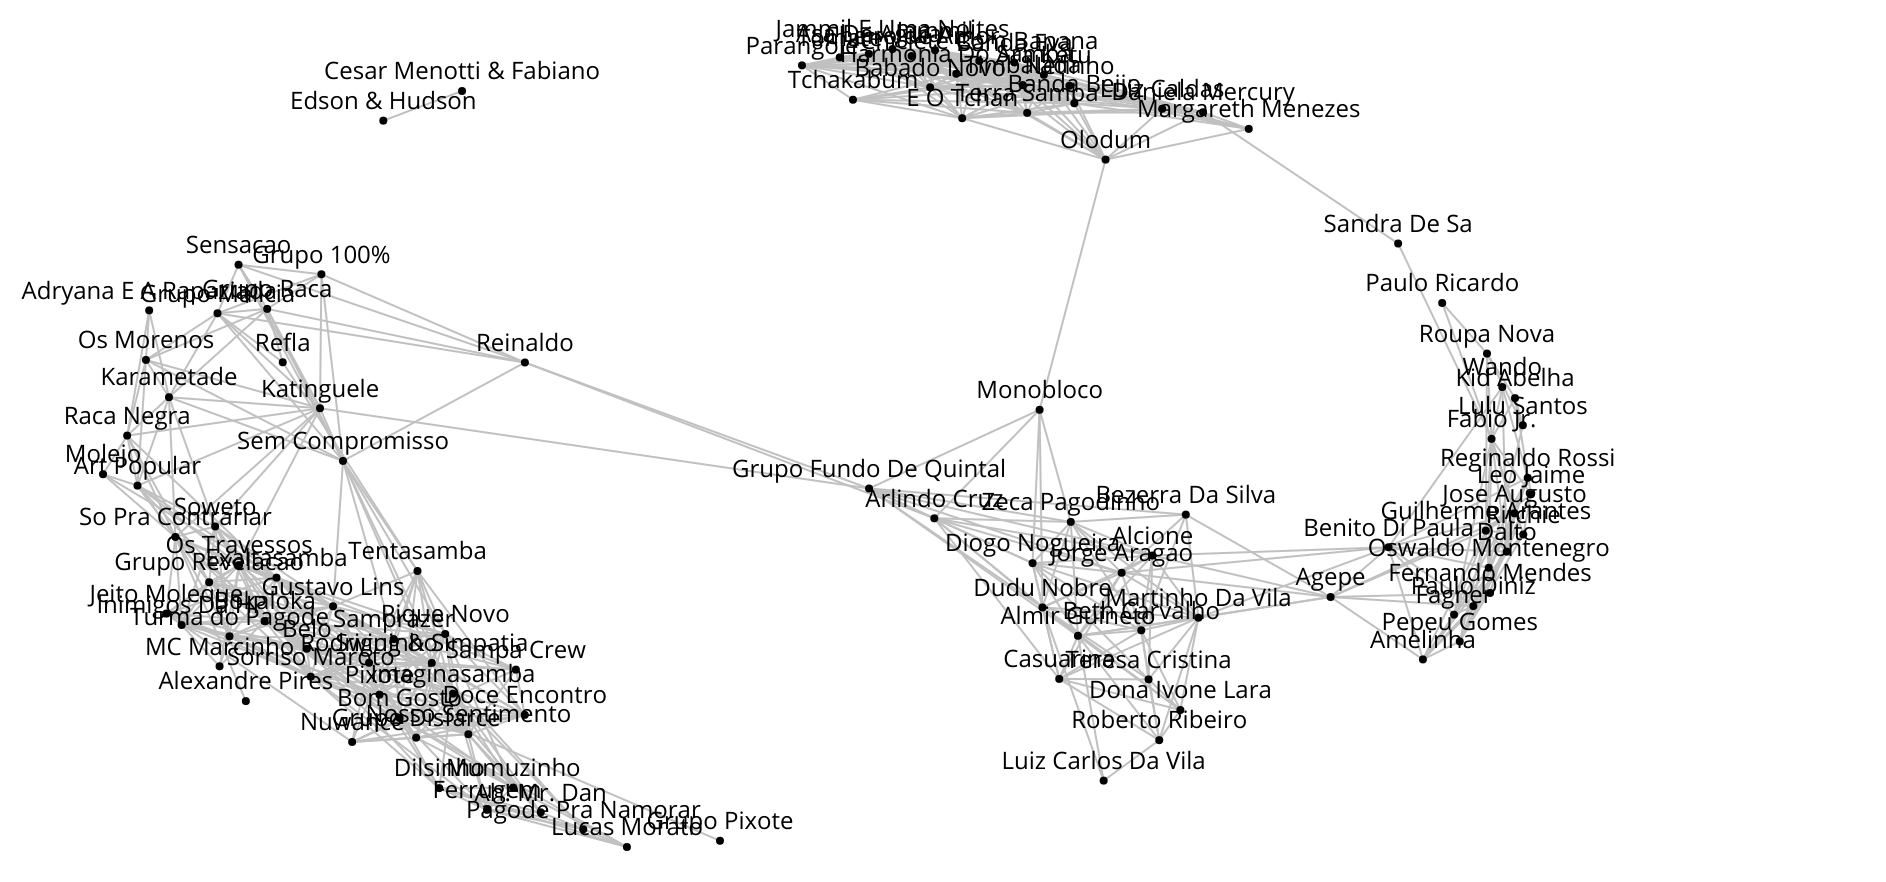
\includegraphics[width=\textwidth]{grafo.png}
	\centering
	\caption{Grafo gerado a partir dos dados recolhidos do Spotify}\label{visina8}
\end{figure}

Pode-se perceber a partir do grafo a divisão de possíveis quatro grupos de artistas relacionados ao Raça Negra. Analisando algumas bandas de cada grupo, uma possível hipótese para essa classificação seria a de subgêneros musicais, como o samba, axé e pagode. No entanto, não há informações o suficiente para chegar a essa conclusão, portanto, a classificação feita para a divisão desses grupos não é clara.

Para identificar-se os artistas responsáveis por conectar esses grupos, foi escolhido a medida de centralidade \textit{betweenness}, por priorizar nós mais presentes em caminhos curtos entre outros dois nós.

\section{Resultados}
Após a análise dos dados utilizando o método  \textit{betweenness}, pode-se chegar em algumas conclusões dos artistas mais importantes para a conexão entre os grupos relacionados ao Raça Negra. Abaixo uma lista dos dez artistas mais centrais junto com o valor de centralidade dos mesmos:

\begin{enumerate}  
	\item Grupo Fundo De Quintal - 2374
	\item Katinguele - 1968
	\item Monobloco - 1443
	\item Olodum - 1409
	\item Sem Compromisso - 1010
	\item Reinaldo - 804
	\item Benito Di Paula - 629
	\item Agepe - 572
	\item Fabio Jr. - 512
	\item Os Travessos - 497
\end{enumerate}


\section{Conclusão}\label{conclusions}
Por fim, é possível perceber que pode-se utilizar a API do Spotify junto a uma análise de centralidade, usando o método \textit{betweenness}, para encontrar bandas centrais na conexão entre grupos de artistas. A utilização desses resultados, ou mesmo desse método usando outros artistas como caso base, pode resultar em um investimento mais focado na recomendação de um grupo musical diferente à um ouvinte, de modo menos agressivo, com uma transição mais gradual, aumentando a probabilidade da pessoa aprovar a recomendação.

\bibliographystyle{abbrv}
\bibliography{main}

\end{document}
This is never printed
  